\documentclass{article}
\usepackage{amssymb, amsthm, enumitem, microtype, verbatim}
\usepackage[utf8]{inputenc}
\usepackage[margin=1in,top=0.6in,bottom=0.6in]{geometry}
\usepackage[fleqn]{amsmath}

% For syntax highlighting
\usepackage{minted}
\begin{comment}
Install: pip install Pygments
Add "-shell-escape", to vscode:
Open settings, search for "latex-workshop.latex.tools", click "Edit in settings.json", add "-shell-escape" to the pdflatex 
command.
\end{comment}

% For displaying accurate time
\usepackage{datetime}
% For PDF metadata
\usepackage[pdfusetitle]{hyperref}
% For outline
\usepackage{navigator}
% Automatically add section to outline
\newcommand{\mysectionstar}[2][]{%
    \ifthenelse{\equal{#1}{}}%
        {\section*{#2}}% If optional argument is empty
        {\section*[#1]{#2}}% If optional argument is not empty
    \outline{1}{#2}%
}
\newcommand{\mysubsectionstar}[2][]{%
    \ifthenelse{\equal{#1}{}}%
        {\subsection*{#2}}% If optional argument is empty
        {\subsection*[#1]{#2}}% If optional argument is not empty
    \outline{2}{#2}%
}
\newcommand{\mysubsubsectionstar}[2][]{%
    \ifthenelse{\equal{#1}{}}%
        {\subsubsection*{#2}}% If optional argument is empty
        {\subsubsection*[#1]{#2}}% If optional argument is not empty
    \outline{2}{#2}%
}
% For images
\usepackage{graphicx}
\begin{comment}
Usage:
\begin{figure}[H]
\centering
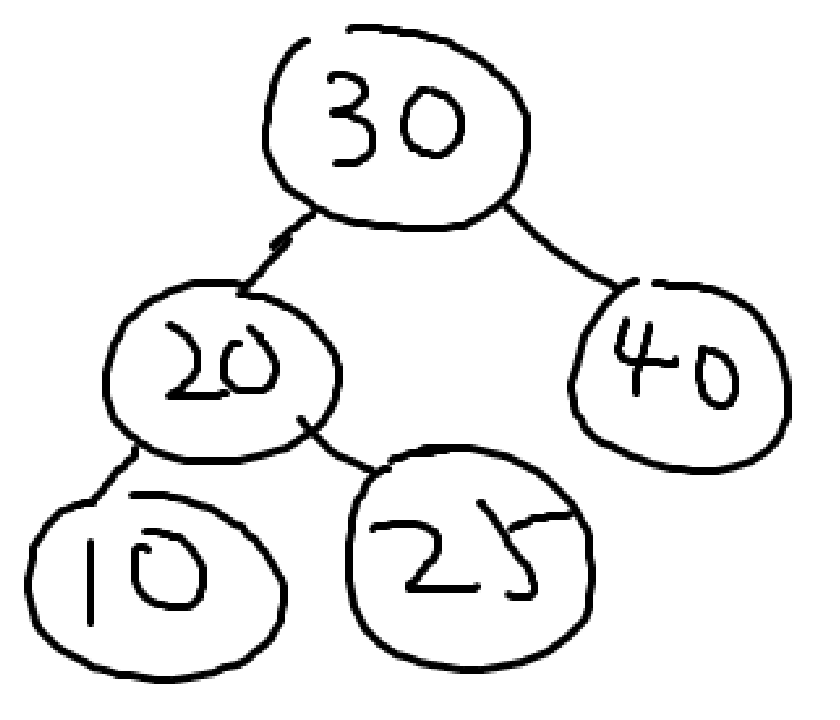
\includegraphics[width=0.4\textwidth]{AVL_Insert_1.png}
\caption{AVL Tree after inserting 30, 20, 40, 10, 25}
\end{figure}
\end{comment}
% For pseudocode
\usepackage{algorithm}
\usepackage{algpseudocode}

\title{COMP2119 Introduction to Data Structures and Algorithms
Assignment 4 - Trees and Sorting Algorithms}
\author{Cheng Ho Ming, Eric (3036216734) [Section 1C, 2024]}
\date{\today \ \currenttime}

\begin{document}
\maketitle

\mysectionstar{Question 1}
\mysubsectionstar{(a)}
\begin{minted}[samepage]{python3}
class BinarySearchTree:
    TreeNode rootNode = None
    # The insert method to support adding tree nodes into the tree
    Function Insert(TreeNode newTreeNode, TreeNode root=rootNode):
        if root is None:
            root = newTreeNode
        else:
            if root.value > newTreeNode.value:
                # Insert new TreeNode into left subtree
                if root.left is None:
                    root.left = newTreeNode
                else:
                    Insert(newTreeNode, root.left)
            else if root.value < newTreeNode.value:
                # Insert new TreeNode into right subtree
                if root.right is None:
                    root.right = newTreeNode
                else:
                    Insert(newTreeNode, root.right)
            else:
                # Should not happen, as we assume the values of all tree nodes are distinct.
\end{minted}

\newpage

\mysubsectionstar{(b)}

\mysubsubsectionstar{(i)}

Given that a node can be a descendant of itself (a.k.a. not required a proper descendant), the lowest common ancestor (denote as $c$) of node $a$ and node $b$ must satisfy the following conditions:


((a.value $<$ b.value) $\rightarrow$ (a.value $<$ c.value $\leq$ b.value)) $\cup$ ((a.value $>$ b.value) $\rightarrow$ (a.value $\geq$ c.value $>$ b.value)) $\cup$ (a.value = b.value = c.value)


The algorithm in pseudocode is:

\begin{minted}[samepage]{python3}
class BinarySearchTree:
    # The method to find the lowest common ancestor of two nodes
    Function FindLowestCommonAncestor(TreeNode a, TreeNode b, TreeNode c=rootNode):
        # If the two given nodes are the same, return the node itself as the lowest common ancestor
        if a.value == b.value:
            return a
        # Ensure that a.value < b.value
        else if a.value > b.value:
            return FindLowestCommonAncestor(b, a, c)
        # c is too large (not the lowest common ancestor)
        # "reduce" the value of c by moving to the left subtree
        else if c.value > b.value:
            return FindLowestCommonAncestor(a, b, c.left)
        # c is too small (not the lowest common ancestor)
        # "increase" the value of c by moving to the right subtree
        else if c.value < a.value:
            return FindLowestCommonAncestor(a, b, c.right)
        else:
            return c
\end{minted}

\mysubsubsectionstar{(ii)}

\begin{minted}[samepage]{python3}
class BinarySearchTree:
    Function GetHeight(TreeNode node):
        if node is None:
            return 0
        else:
            return 1 + max(GetHeight(node.left), GetHeight(node.right))

    Function IsAVLtree(TreeNode root=rootNode):
        # If the tree is empty, it is an AVL tree
        if root is None:
            return True
        # Check if the tree is balanced
        if abs(GetHeight(root.left) - GetHeight(root.right)) > 1:
            return False
        # Check if the left subtree is an AVL tree
        if not IsAVLtree(root.left):
            return False
        # Check if the right subtree is an AVL tree
        if not IsAVLtree(root.right):
            return False
        return True

\end{minted}


\mysectionstar{Question 2}

\mysubsectionstar{(1) Insert the values: 30, 20, 40, 10, 25}

\begin{figure}[H]
\centering
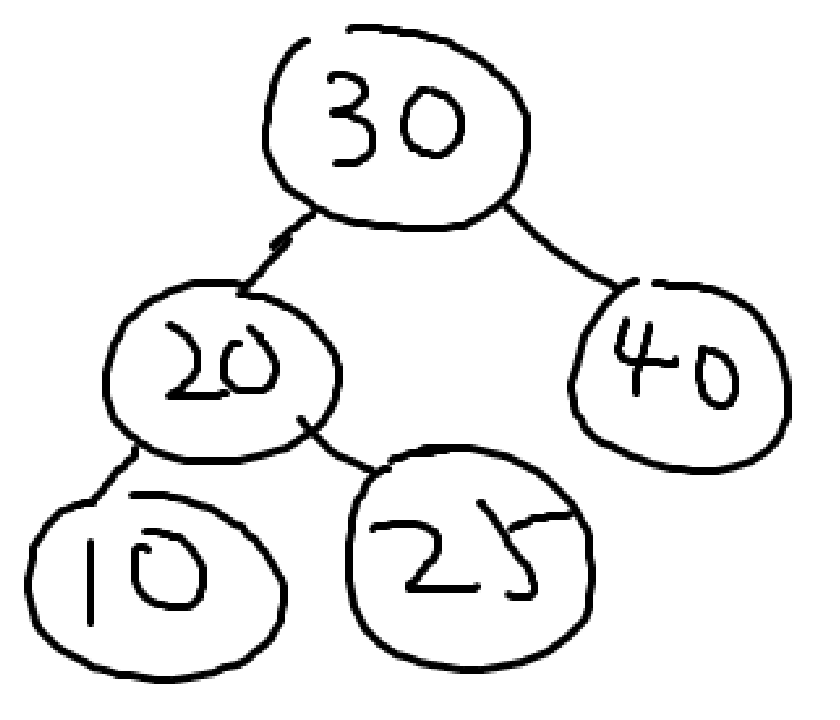
\includegraphics[width=0.4\textwidth]{AVL_Insert_1.png}
\caption{AVL Tree after inserting 30, 20, 40, 10, 25}
\end{figure}

\mysubsectionstar{(2) Insert the value: 5}

\begin{figure}[H]
\centering
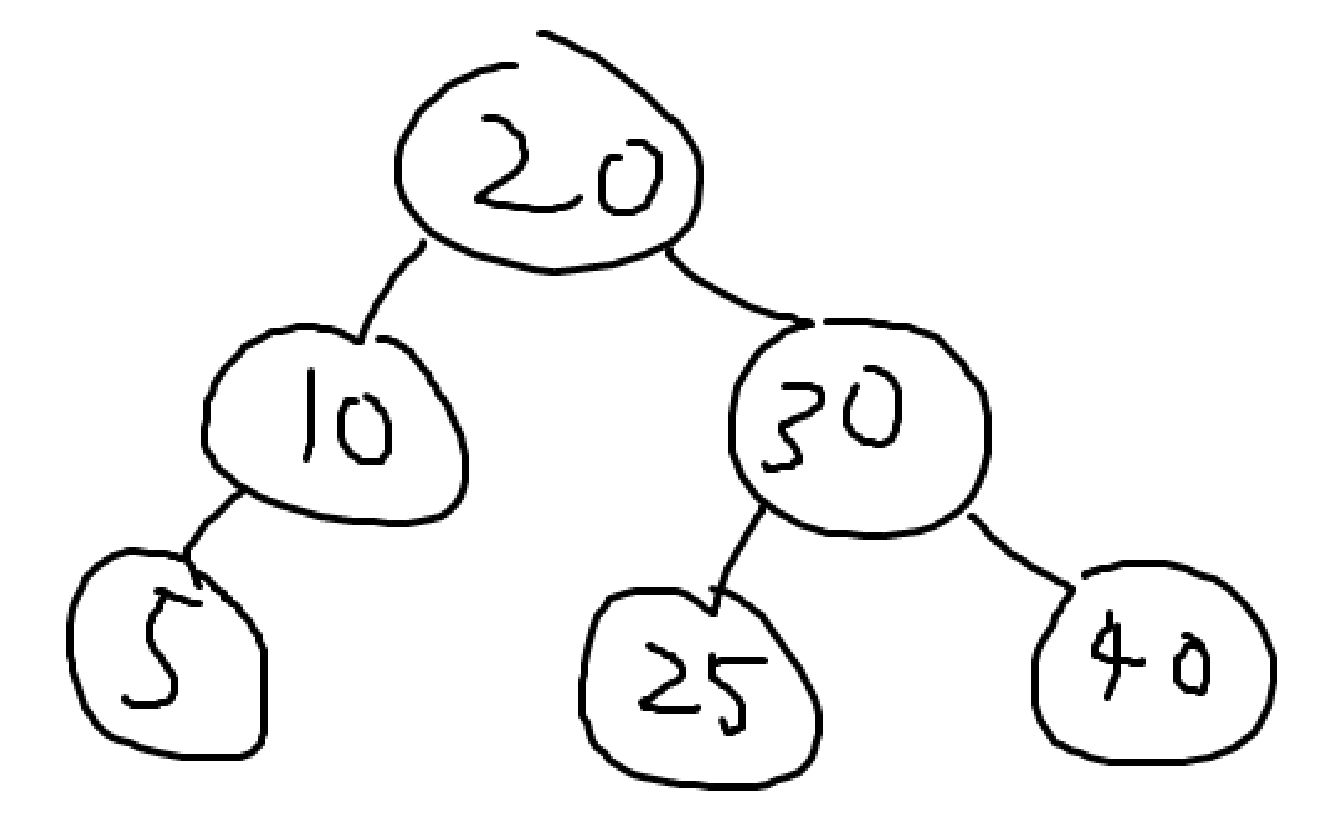
\includegraphics[width=0.4\textwidth]{AVL_Insert_2.png}
\caption{AVL Tree after inserting 5}
\end{figure}

\mysubsectionstar{(3) Delete the value: 30}

\begin{figure}[H]
\centering
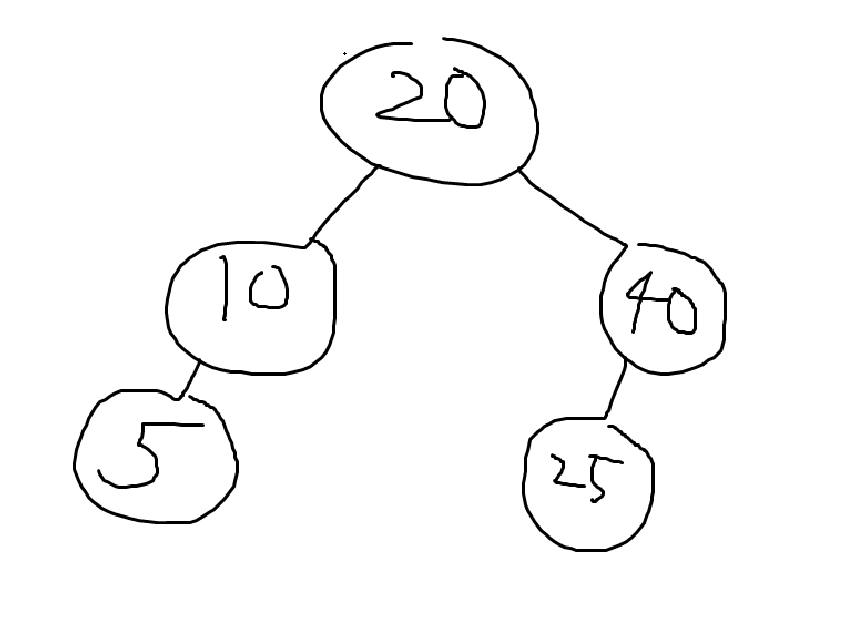
\includegraphics[width=0.4\textwidth]{AVL_Delete.png}
\caption{AVL Tree after deleting 30}
\end{figure}

\mysectionstar{Question 3}

\mysubsectionstar{(a)}

\mysubsubsectionstar{(i)}

$O(n)$

\mysubsubsectionstar{(ii)}

$O(n\log n)$

\mysubsubsectionstar{(iii)}

$O(n^2)$

\mysubsubsectionstar{(iv)}

$O(n^2)$

\mysubsubsectionstar{(v)}

$O(n\log n)$

\mysubsectionstar{(b)}

\mysubsubsectionstar{(i)}

\begin{algorithm}[H]
    \caption{pseudocode that sorts the array in ascending order in O(n) time and O(1) extra space.}
    \begin{algorithmic}
    \Function{Reorder}{$S$}
        \State $nextNegOne \gets 0$
        \State $current \gets 0$
        \State $lastPosOne \gets \text{length}(S) - 1$
        \While{$current \leq lastPosOne$}
            \If{$S[current] = -1$}
                \State \text{Swap}$(S[nextNegOne], S[current])$
                \State $nextNegOne \gets nextNegOne + 1$
                \State $current \gets current + 1$
            \ElsIf{$S[current] = 0$}
                \State $current \gets current + 1$
            \Else \Comment{$S[current] = 1$}
                \State \text{Swap}$(S[current], S[lastPosOne])$
                \State $lastPosOne \gets lastPosOne - 1$
            \EndIf
        \EndWhile
    \EndFunction
\end{algorithmic}
\end{algorithm}

\mysubsubsectionstar{(ii)}

The $nextNegOne$ variable is used to keep track of the next position to place the next -1. The $current$ variable is used to iterate through the array. The $lastPosOne$ variable is used to keep track of the last position to place the next 1. The algorithm iterates through the entire array, and if the current element is -1, it swaps the current element with the element at the $nextNegOne$ position, increases $nextNegOne$ and $current$ by 1. If the current element is 0, it increases $current$ by 1. If the current element is 1, it swaps the current element with the element at the $lastPosOne$ position, and reduces $lastPosOne$.

Since the algorithm will iterate the entire array only once no matter what (for any value of $S[current]$, either $current$ or $lastPosOne$ will be increased or decreased by 1). Therefore, the time complexity is $O(n)$. Three variables are used to store the positions, and recursion is not used, so the space complexity is $O(1)$.

\mysectionstar{Question 4}

\begin{minted}[samepage]{cpp}
class MedianFinder {
    private:
        // Max heap to store the smaller half of the numbers
        std::priority_queue<int, std::vector<int>, std::less<int>> maxHeap;
        // Min heap to store the larger half of the numbers
        std::priority_queue<int, std::vector<int>, std::greater<int>> minHeap;
    public:
        MedianFinder() {}
        
        void addNum(int num) {
            maxHeap.push(num);
            // elements in minHeap should be greater or equal to elements in maxHeap
            minHeap.push(maxHeap.top());
            maxHeap.pop();

            if (minHeap.size() > maxHeap.size()) {
                maxHeap.push(minHeap.top());
                minHeap.pop();
            }
        }
        
        double findMedian(void) {
            // There are odd number of elements
            if (maxHeap.size() > minHeap.size()) {
                return maxHeap.top();
            }
            // There are even number of elements
            return (maxHeap.top() + minHeap.top()) / 2.0;
        }
};
\end{minted}

For the $addNum$ method, since the priority queue is implemented as a binary heap, the time complexity of adding an element (.push()) is $O(\log n)$, where $n$ is the number of elements in the heap. The time complexity of removing the top element (.pop()) is also $O(\log n)$. Therefore, the time complexity of the $addNum$ method is $O(\log n)$.

For the $findMedian$ method, since the top element for each of the heap is located at the root of the heap, the time complexity of getting the top element (.top()) is $O(1)$. Therefore, the time complexity of the $findMedian$ method is $O(1)$.


\end{document}
